\documentclass{article}
% \usepackage[margin=1in,footskip=0.25in]{geometry}
\usepackage{hyperref}
\usepackage{graphicx}
\usepackage[T1]{fontenc}
\usepackage{listings}
\usepackage{xcolor}
 
\definecolor{codegreen}{rgb}{0,0.6,0}
\definecolor{codegray}{rgb}{0.5,0.5,0.5}
\definecolor{codepurple}{rgb}{0.58,0,0.82}
\definecolor{backcolour}{rgb}{0.95,0.95,0.92}
 
\lstdefinestyle{mystyle}{
    backgroundcolor=\color{backcolour},   
    commentstyle=\color{codegreen},
    keywordstyle=\color{magenta},
    numberstyle=\tiny\color{codegray},
    stringstyle=\color{codepurple},
    basicstyle=\ttfamily\footnotesize,
    breakatwhitespace=false,         
    breaklines=true,                 
    captionpos=b,                    
    keepspaces=true,                 
    numbers=left,                    
    numbersep=5pt,                  
    showspaces=false,                
    showstringspaces=false,
    showtabs=false,                  
    tabsize=2
}
 
\lstset{style=mystyle}


\usepackage[margin=1in,footskip=0.25in]{geometry}
\usepackage{hyperref}
\usepackage{graphicx}
\usepackage[T1]{fontenc}
\usepackage{listings}
\usepackage{xcolor}
 
\definecolor{codegreen}{rgb}{0,0.6,0}
\definecolor{codegray}{rgb}{0.5,0.5,0.5}
\definecolor{codepurple}{rgb}{0.58,0,0.82}
\definecolor{backcolour}{rgb}{0.95,0.95,0.92}
 
\lstdefinestyle{mystyle}{
    backgroundcolor=\color{backcolour},   
    commentstyle=\color{codegreen},
    keywordstyle=\color{magenta},
    numberstyle=\tiny\color{codegray},
    stringstyle=\color{codepurple},
    basicstyle=\ttfamily\footnotesize,
    breakatwhitespace=false,         
    breaklines=true,                 
    captionpos=b,                    
    keepspaces=true,                 
    numbers=left,                    
    numbersep=5pt,                  
    showspaces=false,                
    showstringspaces=false,
    showtabs=false,                  
    tabsize=2
}
 
\lstset{style=mystyle}

\usepackage[T1]{fontenc}

\begin{document}

\title{
{\textbf{CS591S1 Project
: Main Report}\\
\large{Explore the Utility in Differentially Private Bayesian Inference}}
}
\author{Jiawen Liu\\
Collaborators: none.}

\date{}
\maketitle
\tableofcontents
%   
\newpage
%
\section{Abstract}
This project focuses on protecting the data privacy in Bayesian analysis process, especially in a differentially private manner.
It starts from existing literatures, summarized popular differentially private Bayesian inference models and their main results in terms of utility under different problem settings.
Then this project studied the connections between these differentially private Bayesian inference models,
and their common utility properties. At the end, we implemented some algorithms proposed in these literatures and compared their results.
%
%
%
\paragraph{Keywords:} data analysis, Bayesian inference, differential privacy, utility optimization, utility trade-off.
%
%
\section{Introduction.}
Modern data analysis techniques have enabled significant
advances in a variety of applications in medicine, finance,
social science, and transportation. Privacy risk occurs when individual users contributes their data, in order to obtain better
services, these applications need large amounts of users’ data. 
Differential privacy was proposed a decade ago to address privacy concerns in these situations, and is now the standard for privacy-preserving data analysis.
While the privacy is always achieved at the expense of sacrificing utility, the trade-off between privacy and utility comes to the light.
Since most of the statistical applications are driven by Bayesian inference, this project will focus on the utility and privacy for differentially private Bayesian inferences.
This is a standard statistical tool in which a prior distribution is combined
with a sample of observed data in order to estimate a new posterior distribution.

The goal of this project is to explore the connections between differentially private Bayesian
inference models, in terms of utility and privacy, under different restrictions and different accuracy measurements (KL divergence, the Hellinger
distance, $l_k$ norm, etc.) over posterior distributions.
%
%

This project builds on some recent surprising works (\cite{ghosh2012universally}, \cite{zhang2016differential}, \cite{bernstein2020noise}) showing the optimality of differentially private Bayesian inference under specific restrictions. 
In this line of work, some proved the best known utility bound and some others proved the universally optimal.
% 
Thus the technique core of this project is to study the connections between these optimizations. 
Especially, there are many other works (\cite{bernstein2019differentially}) on differentially private Bayesian inference that haven't shown optimality.   
From the fundamental perspective, this project study their common utility properties.
%
\paragraph{Contributions.}
This project will systemically study existing differentially private Bayesian inference works in terms of their pre-assumptions/restrictions, structures, utilities and privacy.

\begin{itemize}
	\item Summary of existing structures of differentially private Bayesian inference works under different specifications.
%
	\item Discussion of the connections between utility optimality of different differentially private Bayesian inference structures. 
%	
	\item Extension of one existing model onto another model and experimental results.
%
\end{itemize}

\section{Preliminaries}
\paragraph{Bayesian Inference.}
Given a prior belief $\Pr(\theta)$ on some parameter $\theta$,
and an observation $\dataobs$, the posterior distribution on $\theta$
given $\dataobs$ is defined by Bayes' Theorem as:
\[
  \Pr(\theta | \dataobs) = \frac{\Pr(\dataobs | \theta) \cdot \Pr(\theta)}{\Pr(\dataobs)}
\]
where the expression $\Pr(\dataobs | \theta)$ denotes the
\emph{likelihood} of observing $\dataobs$ under a value of
$\theta$. 
% Since we consider $\dataobs$ to be fixed, the likelihood is
% a function of $\theta$.
% For the same reason $\Pr(\dataobs)$ is a constant independent of $\theta$.
% Usually in statistics the prior distribution $\Pr(\theta)$ is chosen so that it represents
% the initial belief on $\theta$, that is, when no data has been
% observed. In practice though,
In parametric statistics, prior distributions and likelihood functions are usually chosen so that the posterior
belongs to the same \emph{family} of distributions as the prior. In this case we say that the prior
is conjugate to the likelihood function. Use of a conjugate prior
simplifies calculations and allows for inference to be performed in a
recursive fashion over the data. This approach is implemented in a
precise or approximate way in the compiler of several
probabilistic programming languages~\cite{BartheFGAGHS16}.
%
%
\paragraph{Exponential Family.}
The Bayesian Inference in an exponential family is considered in this project. Given the same setting as above, the exponential family in natural parameterization has density:
%
\[
	\Pr(x | \theta) = h(x) \exp(\theta^{T} t(x) - A(\theta)),
\]
%
where $\theta$ are the natural parameters, $t(x)$ is the sufficient statistic,
$A(\theta) = \int h(x) \exp(\theta^T t(x))$
is the log-partition function, and $h(x)$ is the base measure.
The density of the full data is
\[
	\Pr(\dataobs | \theta) = 
	h(\dataobs) \exp(\theta^{T} t(\dataobs) - nA(\theta)),
\]
%
where $h(\dataobs) = \prod h(\dataobs_i)$ and 
$t(\dataobs) = \sum t(\dataobs_i)$.
%
Every exponential family distribution havs a conjugate prior distribution $p(\theta; \lambda)$
with hyperparameters $\lambda$. 
A conjugate prior has the property that, if it is used as the prior, 
then the posterior belongs to the same family, i.e., $\Pr(\theta | \dataobs; \lambda) = p(\theta;\lambda')$ 
for some $\lambda'$ that depends only on $\lambda, n$ and the sufficient statistics $s$.
%
Our following research will focus on some specific models in this exponential family. 

% \paragraph{Differential Privacy.}
% %
% %
% \emph{Differential privacy}~\cite{dwork2006} is a quantitative notion
% of data privacy guaranteeing  a bound on the that changing the input of a mechanism slightly only reflects
% in a controlled and bounded way on the output distribution. 
% Formally, the $\epsilon$ parameter
% controls how much two outputs starting from \emph{close} inputs can differ. When two inputs are close we call them \emph{adjacent}.
% By adjacency we usually mean a relation over input databases which includes all the pair of databases which differ by at most one row.
% The formal definition of $\epsilon$-differential privacy follows.
% \begin{defn}
% \label{def_epsilon_dp}
% A randomized mechanism $\mathcal{M}$ with domain $\mathbb{N}^{|\mathcal{X}|}$ and codomain $\range$, is $\epsilon$-differential private, if for all adjacent
% \footnote{Given $\dataobs, \dataobs'\in\{0,1\}^n$  we say that $\dataobs$ and $\dataobs'$ are adjacent and we write, iff
% $\sum_{i}^{n}\iverson{x_i = x'_i }\leq 1$. } $\dataobs, \dataobs' \in \mathbb{N}^{|\mathcal{X}|}$ and all $\mathcal{S} \subseteq \range$:
% \begin{equation*}
% \Pr[\mathcal{M}(\dataobs) \in \mathcal{S}] \leq e^\epsilon \Pr[\mathcal{M}(\dataobs') \in \mathcal{S}].
% \end{equation*}

% \end{defn}


% It is possible to achieve $\epsilon$-differential privacy through use and composition of
% a few basic components. Some of these components are now reviewed.
%
%
\section{Differentially Private Bayesian Inference Models}
%
This section introduced three kind of differentially private Bayesian inference Models we will study in detail in following works as shown in Figure \ref{fig_pinfermodel}. 
\begin{figure*}[t!]
    \centering
    \begin{subfigure}[t]{0.3\textwidth}
        \centering
        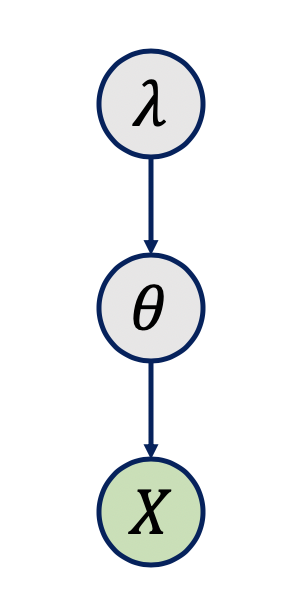
\includegraphics[height=1.2in]{nonp.png}
        \caption{Non Private Bayesian Inference}
    \end{subfigure}%
    ~ 
    \begin{subfigure}[t]{0.3\textwidth}
        \centering
        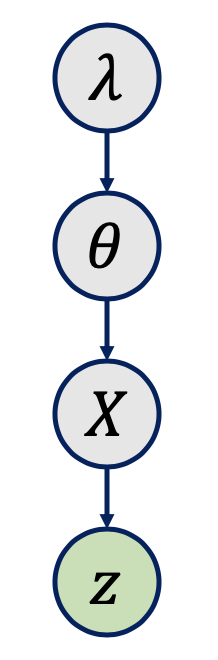
\includegraphics[height=1.2in]{pinfer}
        \caption{Private Bayesian Inference on Data}
    \end{subfigure}
    ~ 
    \begin{subfigure}[t]{0.3\textwidth}
        \centering
        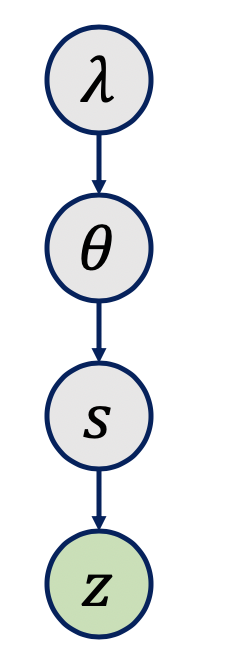
\includegraphics[height=1.2in]{pinferons}
        \caption{Private Bayesian Inference on Sufficient Statistics}
    \end{subfigure}
    \caption{Private Bayesian Inference Model}
    \label{fig_pinfermodel}
\end{figure*}
\subsection{Non-private Inference}
%
As shown in Figure \ref{fig_pinfermodel}(a), the non-private inference graph starts
from the hyper-parameter following by the Bayesian inference process in exponential family.
%
Then it will directly release the full data without any manipulation on data.

\subsection{Private Inference over Data}
%
As shown in Figure \ref{fig_pinfermodel}(b), 
the private inference over data start with the same pre-procedure as non-private model with the same hyper-parameter and prior distribution.
%
Then instead of release the data directly, it perform the analysis and release a perturbed quantity $z$.
%
In this way, the noise model due to the release mechanism can be directly accounted for in a probabilistic inference procedure, 
with the intent of producing more principled and higher-utility private analyses.
%
\\
The key insight is that exposing the details of the release mechanism does not harm the differential privacy guarantee. 
Given release mechanisms are made public,
the knowledge of the mechanism defines the conditional distribution $\Pr(z |\dataobs)$,
which can be combined with the generative data model, $\Pr(\dataobs | \theta)$, to form a new likelihood distribution on data:
\[
\Pr(z | \theta) = 
\int
\Pr(\dataobs | \theta)
\Pr(z |\dataobs) d \dataobs.
\] 
%
Thus the main technique developed under this model is to form approximations of this integral and obtain either a closed form or a tractable sampling procedure.

\subsection{Private Inference over Sufficient Statistics}
%
As shown in Figure \ref{fig_pinfermodel}(c), instead of working with individual data directly,
this model works with the sufficient statistics,
where the sufficient statistics are quantities
that capture all information about the model parameters (\cite{foulds2016theory}, \cite{vu2009differential}).
%
In this model, noises are added to these sufficient statistics and then Bayesian inference analysis are performed on these noisy statistics where the analysis results will finally be released. 
%
\\
%
This project will study some specific problems and algorithms mainly under this model and then focus on the connections and difference between the two models.
%
\section{Private Bayesian Inference under Different Problem Settings}
%

\subsection{Counting Query Model \texorpdfstring{\cite{ghosh2012universally}}{}}
%

\subsubsection{Problem Setting}
%
Following the model in Figure \ref{fig_pinfermodel}(c), this section studied under the setting: 
1) The sufficient statistics are results from counting queries and 
2) the randomization mechanism of releasing the noisy statistics
is adding discrete noises to query results by geometric distribution. 
There is no specific restriction on the inference model after the release of sufficient statistics.
%
Below are some formal definitions which will be used in this model.
%
%
%
\[
\begin{array}{lcl}
	d \in D^n 
	& : &
	\mbox{The data base}.\\
	f : D^n \rightarrow [N]
	& : & \mbox{the counting query, It's result is a sufficient statistic.}\\
	\mathcal{A}: [N] \rightarrow R
	& : & \mbox{the randomization mechanism}\\
	p_i
	& : & \mbox{prior probability distribution over the query results } i \in [N]\\
	l(i; r)
	& : & \mbox{loss function $l$, over query results $i$ and mechanism output $r$}
\end{array}
\]
%
%
\begin{defn}[Counting Query]
A count query $f$ takes a database $d \in D^n$ as input and returns the result $f(d) \in N = \{0, \cdots ,n\}$ that is the number of rows that satisfy a fixed, non-trivial predicate on the domain D.
\end{defn}
%
\begin{defn}[$\epsilon$-Geometric Mechanism]
When the true query result is $f(d)$, the mechanism outputs $f(d)+Z$. Z is a random variable distributed as a two-sided geometric distribution: 
$Pr[Z = z] = \frac{1 - e^{-\epsilon}}{1 + e^{-\epsilon}} e^{-\epsilon|z|}$
for every integer $z$. The details of this mechanism is shown in Algorithm \ref{alg_geo}, where $\mathcal{A}: [N] \rightarrow R $.
%
\begin{algorithm}
\caption{$\epsilon$-Geometric Algorithm $\mathcal{A}$}
\label{alg_geo}
\begin{algorithmic}
\REQUIRE database $d \in D^n$.
\STATE {\bf Initialize} counting queries $f : D^n \rightarrow \{0, \cdots ,n\}$,  privacy budget $\epsilon$.
\STATE  {\bf let} $i = f(d)$; 
\STATE  {\bf let} $r = \mathcal{A}(i)$; 
\COMMENT {$\mathcal{A}(i)$ : $i + (z \leftarrow Geo(\epsilon))$}
\STATE  \COMMENT{geo mech $\mathcal{A}(i)$ sample a random value $z$ from $\epsilon$-Geometric distribution and added to query result $i$.}
\RETURN $r$.
\end{algorithmic}
\end{algorithm} 
%
\end{defn}
%
In order to prove the universal optimal, it is necessary to clarify the utility model under which the optimal is achieved. 
So we have following 3 definition where 
the \emph{preference} and \emph{side information} are defined firstly in order to model the utility.
%
\begin{defn}[preference]
The preference of user is defined by a loss function: $l(i; r): [N] * R \rightarrow R'$,
where $i \in [N]$ is the counting query result, $r \in R$ is the result from mechanism $\mathcal{A}$.
The only constrains on the loss function are nonnegative and nondecreasing in $|i - r|$ for each fixed $i$. 
\end{defn}

\begin{defn}[side information]
The side information is simply the prior distribution $p_i$ over the query results $i$.
\end{defn}

\begin{defn}[Utility Model]
In order to achieve universally optimality over all potential users, utility model is defined independent
of \emph{preference} and \emph{side information} as follows:
\[
\sum_{i \in [1,\ldots, n]}p_i \sum_{r \in R}
Pr[\mathcal{A}(i) = r] \cdot l(i;r).
\]
which is actually expected loss over the randomness of the mechanism and the prior.
%
\end{defn}
%
%
%
%
\subsubsection{Main Theorem}
%
\begin{thm}[\cite{ghosh2012universally}]
for each fixed count query and differential privacy level,
there is a geometric mechanism 
$M$ that is simultaneously expected loss-minimizing for every possible user,
subject to the differential privacy constraint.
\end{thm}
%
In order to prove this main theorem, there are following reductions between this problem and other problems:
\paragraph{Equivalence Between Private Inference and $\epsilon$-Geometric mechanism}
%
This equivalence comes from the observation that: the post-processing will only reduce the information loss.
So we can have following equivalence:
Every private inference process can be factored into a user-independent ($\epsilon$-geometric mechanism) followed by a user-dependent post-processing step.
Because the post-processing will only reduce the information loss, 
therefore it is sufficient to prove the user-independent ($\epsilon$-geometric mechanism) 
optimal in order to prove any private inference process optimal. 

\paragraph{Reduction to Linear Programming Problem}
Now we only need to care about the user-independent ($\epsilon$-geometric mechanism) and prove its optiamlity. 
This problem is further reduce
the problem of determining the differentially private mechanism that minimizes expected loss
as a solution to a linear program (LP) as following. It is further proved by Lemma \ref{lem:LP_opt} that there is always a optimal solution to this LP problem.
%
\[
    \begin{array}{rl}
    \mbox{minimize} 
    & \sum_{i \in [1,\ldots, n]}p_i \sum_{r \in R}
    Pr[\mathcal{A}(i) = r] \cdot l(i;r)\\
    Pr[\mathcal{A}(i) = r]  
    - e^{\epsilon}Pr[\mathcal{A}(i + 1) = r] \geq 0
    & \forall r \in N \setminus {n}, i \in N\\
    Pr[\mathcal{A}(i + 1) = r]  
    - e^{\epsilon}Pr[\mathcal{A}(i) = r] \leq 0
    & \forall r \in N \setminus {n}, i \in N\\
    \sum_{r \in R}
    Pr[\mathcal{A}(i) = r] = 1
    & \forall i \in N\\
    Pr[\mathcal{A}(i) = r] \geq 0
    & \forall r \in N \setminus {n}, i \in N\\    
    \end{array}
\]
%
\begin{lem}[\cite{ghosh2012universally}]
\label{lem:LP_opt}
Every user-specific LP (reduced from mechanisms determination as above) has an optimal solution that is a vertex.
\end{lem}

\subsection{InverseGamma-Gaussian Model
\texorpdfstring{\cite{bernstein2019differentially}}{}}
%
\subsubsection{Problem Setting}
%
Again following the model in Figure \ref{fig_pinfermodel}(c), another popular problem studied under this model is Bayesian linear regression in the InverseGamma-Gaussian Model. 
%
Below are some formal definitions which will be used in this model.

%
\begin{defn}[Linear Regression with InverseGamma-Gaussian Model]
The linear regression model are defined with:

The population data: $\dataX \in R^{d \times n}$.

The dependent response data: $\datay \in R^{n}$.

The likelihood model: conditional Gaussian model 
$\datay \sim \normdis(\vtheta^{T} \dataX, \sigma^2)$,
where $\vtheta \in R^d$ are the regression coefficients and
$\sigma^2$ is the error variance.

The point estimation of $\vtheta$: 
$\hat{\vtheta} = (\dataX^T \dataX)^{-1} \dataX^T \datay$, 
i.e., the ordinary least solution.

The conjugate prior: $p(\sigma^2) = \text{InverseGamma}(a_0, b_0 )$ 
and $p(\vtheta | \sigma^2) = \normdis (\vmu_0 , \sigma^2\vLambda_0^{-1})$. 
The joint distribution are defined as:
$p(\vtheta, \sigma^2) = NIG(\vmu_0, \sigma^2\vLambda_0^{-1}, a_0, b_0)$.

The posterior: 
$p(\vtheta, \sigma^2 | \dataX, \datay) = 
NIG (\vmu_n, \sigma^2\vLambda_n^{-1}, a_n, b_n)$, where 
$\vmu_n = (\dataX^T \dataX + \vLambda_0)^{-1}
(\dataX^T \datay + \vmu_0^{T}\vLambda_0)$;
$\sigma^2\vLambda_n^{-1} = \dataX^T \dataX + \vLambda_0$;
$a_n = a_0 + \frac{1}{2}n$;
$b_n = b_0 + \frac{1}{2}(\datay^T\datay 
+ \vmu_0^{T}\vLambda_0 \vmu_0
- \vmu_n^{T}\vLambda_n \vmu_n)$.
\end{defn}

\begin{defn}{Sufficient Statistics}
The sufficient statistics $s$ in this model are:
\[
	s := t(\dataX, \datay) = [\dataX^T \dataX, \dataX^T \datay, \datay^T\datay]
\]
\end{defn}

\begin{defn}[Private Linear Regression Model]
Following the sufficient-statistic perturbation model, we have the noisy sufficient statistics for public release are:
\[
	\dataz = [z_i = s_i + \lap{\delta_s}{0} : s_i \in s]
\]
\end{defn}


\begin{defn}[Utility Measures]
The utility is measured as closeness to the non-private posterior, by maximum mean discrepancy (MMD), a kernel-based statistical test to determine if two sets of samples are drawn from different distributions. It is defined as: given $n$ i.i.d. samples $(p, q) \sim (P \times Q)$, the MMD between distribution of $P$ and $Q$ is
\[
	MMD^2(P, Q) = \frac{1}{n(n - 1)}
	\sum_{i \neq j}^{n}
	(k(p_i, p_j ) + k(q_i, q_j ) 
	- k(p_i, q_j ) - k(p_j , q_i)),
\]
where $k$ is a standard normal kernel in this paper.
\end{defn}
%
%
\subsubsection{Main Result}
%
Instead of trying to prove optimality on existing algorithms or mechanisms, this work focus on designing algorithms which can produce good posterior distributions and perform sampling with higher accuracy.
%

The main results are inference algorithms proposed based on publicly released noisy sufficient statistics $\dataz$. 
It computes a representation of
$ p(\vtheta, \sigma^2 | \dataz) \propto \int_{s}   p( \vtheta, \sigma^2, s, \dataz) ds$ by integrating over the sufficient statistics $s$.

%
%
And the results about utility are shown in experiments measured by MMD defined above.

\subsection{Beta-Binomial Model
\texorpdfstring{\cite{Zhang2017privbayes}}{}}
\label{sec_betabi}
%

\subsubsection{Problem Setting}
%
This model focus on Bayesian inference with Beta-Binomial distribution.
%
Different from previous two models, this model following the second model in Figure \ref{fig_pinfermodel}(b). Instead of working on sufficient statistics, they are working on the data directly and release the private inference result. 

%
Below are some formal definitions which will be used in this model.

\begin{defn}[Beta-Binomial Model]
The Beta-Binomial model is a specific case of Dirichlet-Multinomial model for
categorical data and its restriction to binary data.
That is, we will consider the situation where 
the underlying categorical data is drawn from a multinomial
distribution with parameter the vector $\vtheta\in [0,1]^{k}$. The prior distribution over $\vtheta$
is given by a Dirichlet distribution, $\dirichlet{\valpha}$, for,
$\valpha\in(\mathbb{R}^{+})^{k}$ and $k\in\mathbb{N}$, with p.d.f:
\[
\Pr(\vtheta)=\frac{1}{\mbetaf(\valpha)}\cdot\prod_{i=1}^{k}{\theta_i^{\alpha_i-1}}
\]
where $\mbetaf(\cdot)$ is the generalized beta function.
The data $\dataobs$ is a sequence of $n\in\mathbb{N}$ values
coming from a universe $\datauni$, such that $|\datauni|=k$.
The likelihood function is
$
\Pr(\dataobs|\vtheta)=\prod_{a_i\in\datauni}\theta_{i}^{\Delta \alpha_i},
$
with $\Delta \alpha_i=\displaystyle\sum_{j=1}^{n}\mathbf{1}_{\iverson{x_j=a_i}}$.
Denoting by $\Delta\valpha$ the vector $(\Delta\alpha_1,\dots
\Delta\alpha_k)$ the posterior distribution over $\vtheta$ is
$\dirichlet{\valpha + \Delta \valpha}$, where $+$ denotes the component wise sum of vectors.
In the following we will use the notation $\bysinfer{\valpha,\vtheta,
\dataobs}$ to denote the posterior of this process.
The Beta-Binomial model can be obtained from the Dirichlet-Multinomial
model by fixing $k=2$. 
\end{defn}


\begin{defn}[Laplace Mechanism]
The Laplace mechanism releases a random number drawn from the Laplace distribution with
mean $\mu=q(d)$ and scale $\nu$. Where $q$ is a numeric query on a database $d$.
If $\nu\geq \frac{\Delta_f}{\epsilon}$, with $\Delta_f=\displaystyle\max_{d,d':\adj{d}{d'}}{\lvert f(d_1)-f(d_2)\lvert}$
then the mechanism is $\epsilon$-differentially private.
\end{defn}


\subsubsection{Main Theorem}
The details of their algorithm are defined in Algorithm \ref{alg:lapmech}:
%
\begin{algorithm}
  \caption{Laplace Mechanism based Differentially Private Bayesian Inference}
  \label{alg:lapmech}
  \begin{algorithmic}
  \STATE $\dataobs\in\mathcal{X}^n$, $Beta(a, b)$
  \STATE \quad {\bf let} $(a', b') = (\#\{i | x_i = 1\}, \#\{i | x_i = 0\})$, 
  \STATE \quad  {\bf let} $\tilde{a} = a + \lfloor{(a' - a)+ \lap{0}{\frac{2}{\epsilon}} }\rfloor^n_0$,
  $\tilde{b} = b + \lfloor{(b' - b)+ \lap{0}{\frac{2}{\epsilon}} }\rfloor^n_0$.
  \STATE {\bf return} $(\tilde{a}, \tilde{b})$
  \end{algorithmic}
\end{algorithm}
%
\\
The utility is measured as the distance to the true posterior, by KL-divergence. 
\begin{thm}[Utility Bounds on Posterior]
The loss of utility measured by KL-divergence is no more than:
\[
	\mathcal{O}(2n\ln n)\big[ 1 - \exp(-n\epsilon / 2) \big] + \sqrt{-\mathcal{O}(2 n \ln n) \ln \delta},
\]
with probability at least $1 - \delta$.
\end{thm}
%
%
\section{Connections Between Different Models}
The three models summarized above focus on 3 different aspects of the problem:
\begin{enumerate} 
\item Given the specific counting query and geometric-mechanism, this paper focus on proving the utility optimality by 
1) mapping all possible private mechanism onto this mechanism and 2) then reducing it to a LP problem.
%
\item Given the differentially private sufficient statistics are released publicly, 
the second model focus on designing inference algorithm based on the released sufficient statistics. 
By adopting different approximating ways, they design inference algorithm producing posterior closer to the true posterior.
%
\item The third work is developed under the second private Bayesian inference model (Figure \ref{fig_pinfermodel}(b)) different from the other two works.
They actually performed a naive inference by ignoring the noise added to statistics.
However, can we adopt this problem in the private Bayesian inference over sufficient statistics model (Figure \ref{fig_pinfermodel}(c))?
This gives me the next section.
\end{enumerate}

Additionally, the utilities in the three models are also evaluated in 3 different ways as well as the optimality:
\begin{enumerate} 
\item Only the first counting query model proved the optimality,
by reducing to the famous LP problem and showing the existence of optimal solution.
%
\item The utility in the second linear regression model are only studied by experiments. 
The experimental results shown that their noisy aware inference based on sufficient statistics
have the best utility among all private linear regression algorithms.
They didn't prove the optimal formally but we can still say they are the existing optimal private Bayesian linear regression algorithm.
%
\item In the third work with the Beta-Binomial inference model, the utilities are given by utility bound. This utility bound in terms of KL-divergence is the best know bound for Laplace mechanism.
\end{enumerate}
%

Although the third work theoretically gave the best known utility bound \cite{zhang2016differential}.
This cannot guarantee there is no algorithm or mechanism having better utility.
This gives us room for improvement. 
%
However, the first model indeed proved the optimality and gave no room for improvement.
%
Can we adopt the work in \cite{bernstein2019differentially}, \cite{zhang2016differential}
in the framework of the counting query model?
This gives me the following sections.

%

\section{Beta-Binomial Model V.S. Counting Querying Model}
In order to shown the Beta-Binomial model and Laplace mechanism shown in Section \ref{sec_betabi} can be 
formalized into the counting querying model, we need to shown following mapping:
\[
	\begin{array}{lcl}
	\Delta \alpha : \#\{i |x_i = 1\}
	& \Rightarrow &
	f:\{0, 1\}^d \rightarrow [N] \mbox{: the counting query}\\
	\lfloor \lap(2/\epsilon, 0) \rfloor_0^{n}
	& ? &
	geo(\epsilon) \mbox{: the geometric mechanism}\\
	beta(\alpha, \beta)
	& \Rightarrow &
	p_{i} \mbox{: the prior distribution over the query result (i.e., $\#\{i |x_i = 1\}$) }\\
	KL(P, Q)
	& \Rightarrow &
	l(i; r) \mbox{: the loss function (symmetric and non-increasing w.r.t. $|i - r|$).}
	\end{array}
\]
If the mapping from $\lfloor \lap{0}{2/\epsilon} \rfloor_0^{n}$ to $\lfloor geo(\epsilon) \rfloor_0^{n}$ holds,
then we can have the mapping from the Beta-Binomial model onto the counting query model.
Consequently, 
it indirectly proved that the Laplace algorithm \ref{alg:lapmech} is optimal in this model.

By the p.d.f. of Laplace distribution, we have following probability function:
\[
	Pr[\lfloor \lap{0}{2/\epsilon} \rfloor_0^{n} = z]
	= \frac{1}{2}(e^{-z\epsilon /2} - e^{-(z + 1)\epsilon / 2}).
\]
It is obviously that $\lfloor \lap(2/\epsilon, 0) \rfloor_0^{n}$ have different probability distribution as $\lfloor Geo(\epsilon) \rfloor_0^{n}$ 
($Pr[\lfloor Geo(\epsilon) \rfloor_0^{n} = z] = 
\frac{1 - e^{-\epsilon}}{1 + e^{-\epsilon}} e^{-\epsilon|z|}$).
i.e., the Beta-Binomial model with Laplace mechanism cannot be fully reduce to the counting query model 
with optimal Geometric mechanism.

However, it is still possible we can adopt the Geometric mechanism into the Beta-Binomial model as shown in Algorithm \ref{alg:betabi_geomech}, by simply substituting the Laplace noise with the Geometric noise.

\begin{algorithm}
  \caption{Geometric Mechanism based Differentially Private Bayesian Inference}
  \label{alg:betabi_geomech}
  \begin{algorithmic}
  \STATE $\dataobs\in\mathcal{X}^n$, $Beta(a, b)$
  \STATE \quad {\bf let} $(a', b') = (\#\{i | x_i = 1\}, \#\{i | x_i = 0\})$, 
  \STATE \quad  {\bf let} $\tilde{a} = a + \lfloor{(a' - a)+ Geo({\epsilon}) }\rfloor^n_0$,
  $\tilde{b} = b + \lfloor{(b' - b)+ Geo({{\epsilon}}) }\rfloor^n_0$.
  \STATE {\bf return} $(\tilde{a}, \tilde{b})$
  \end{algorithmic}
\end{algorithm}
%

I compared the two algorithms by experiments. The experimental results shown in Figure \ref{fig_geovslap} verified that adding Laplace noise is not as good as adding Geometric noise. Code is available in appendix as well as github repository: \url{https://github.com/jiawenliu/CS591S1.git}.  
\begin{figure*}[t!]
    \centering
    \begin{subfigure}[t]{0.3\textwidth}
        \centering
        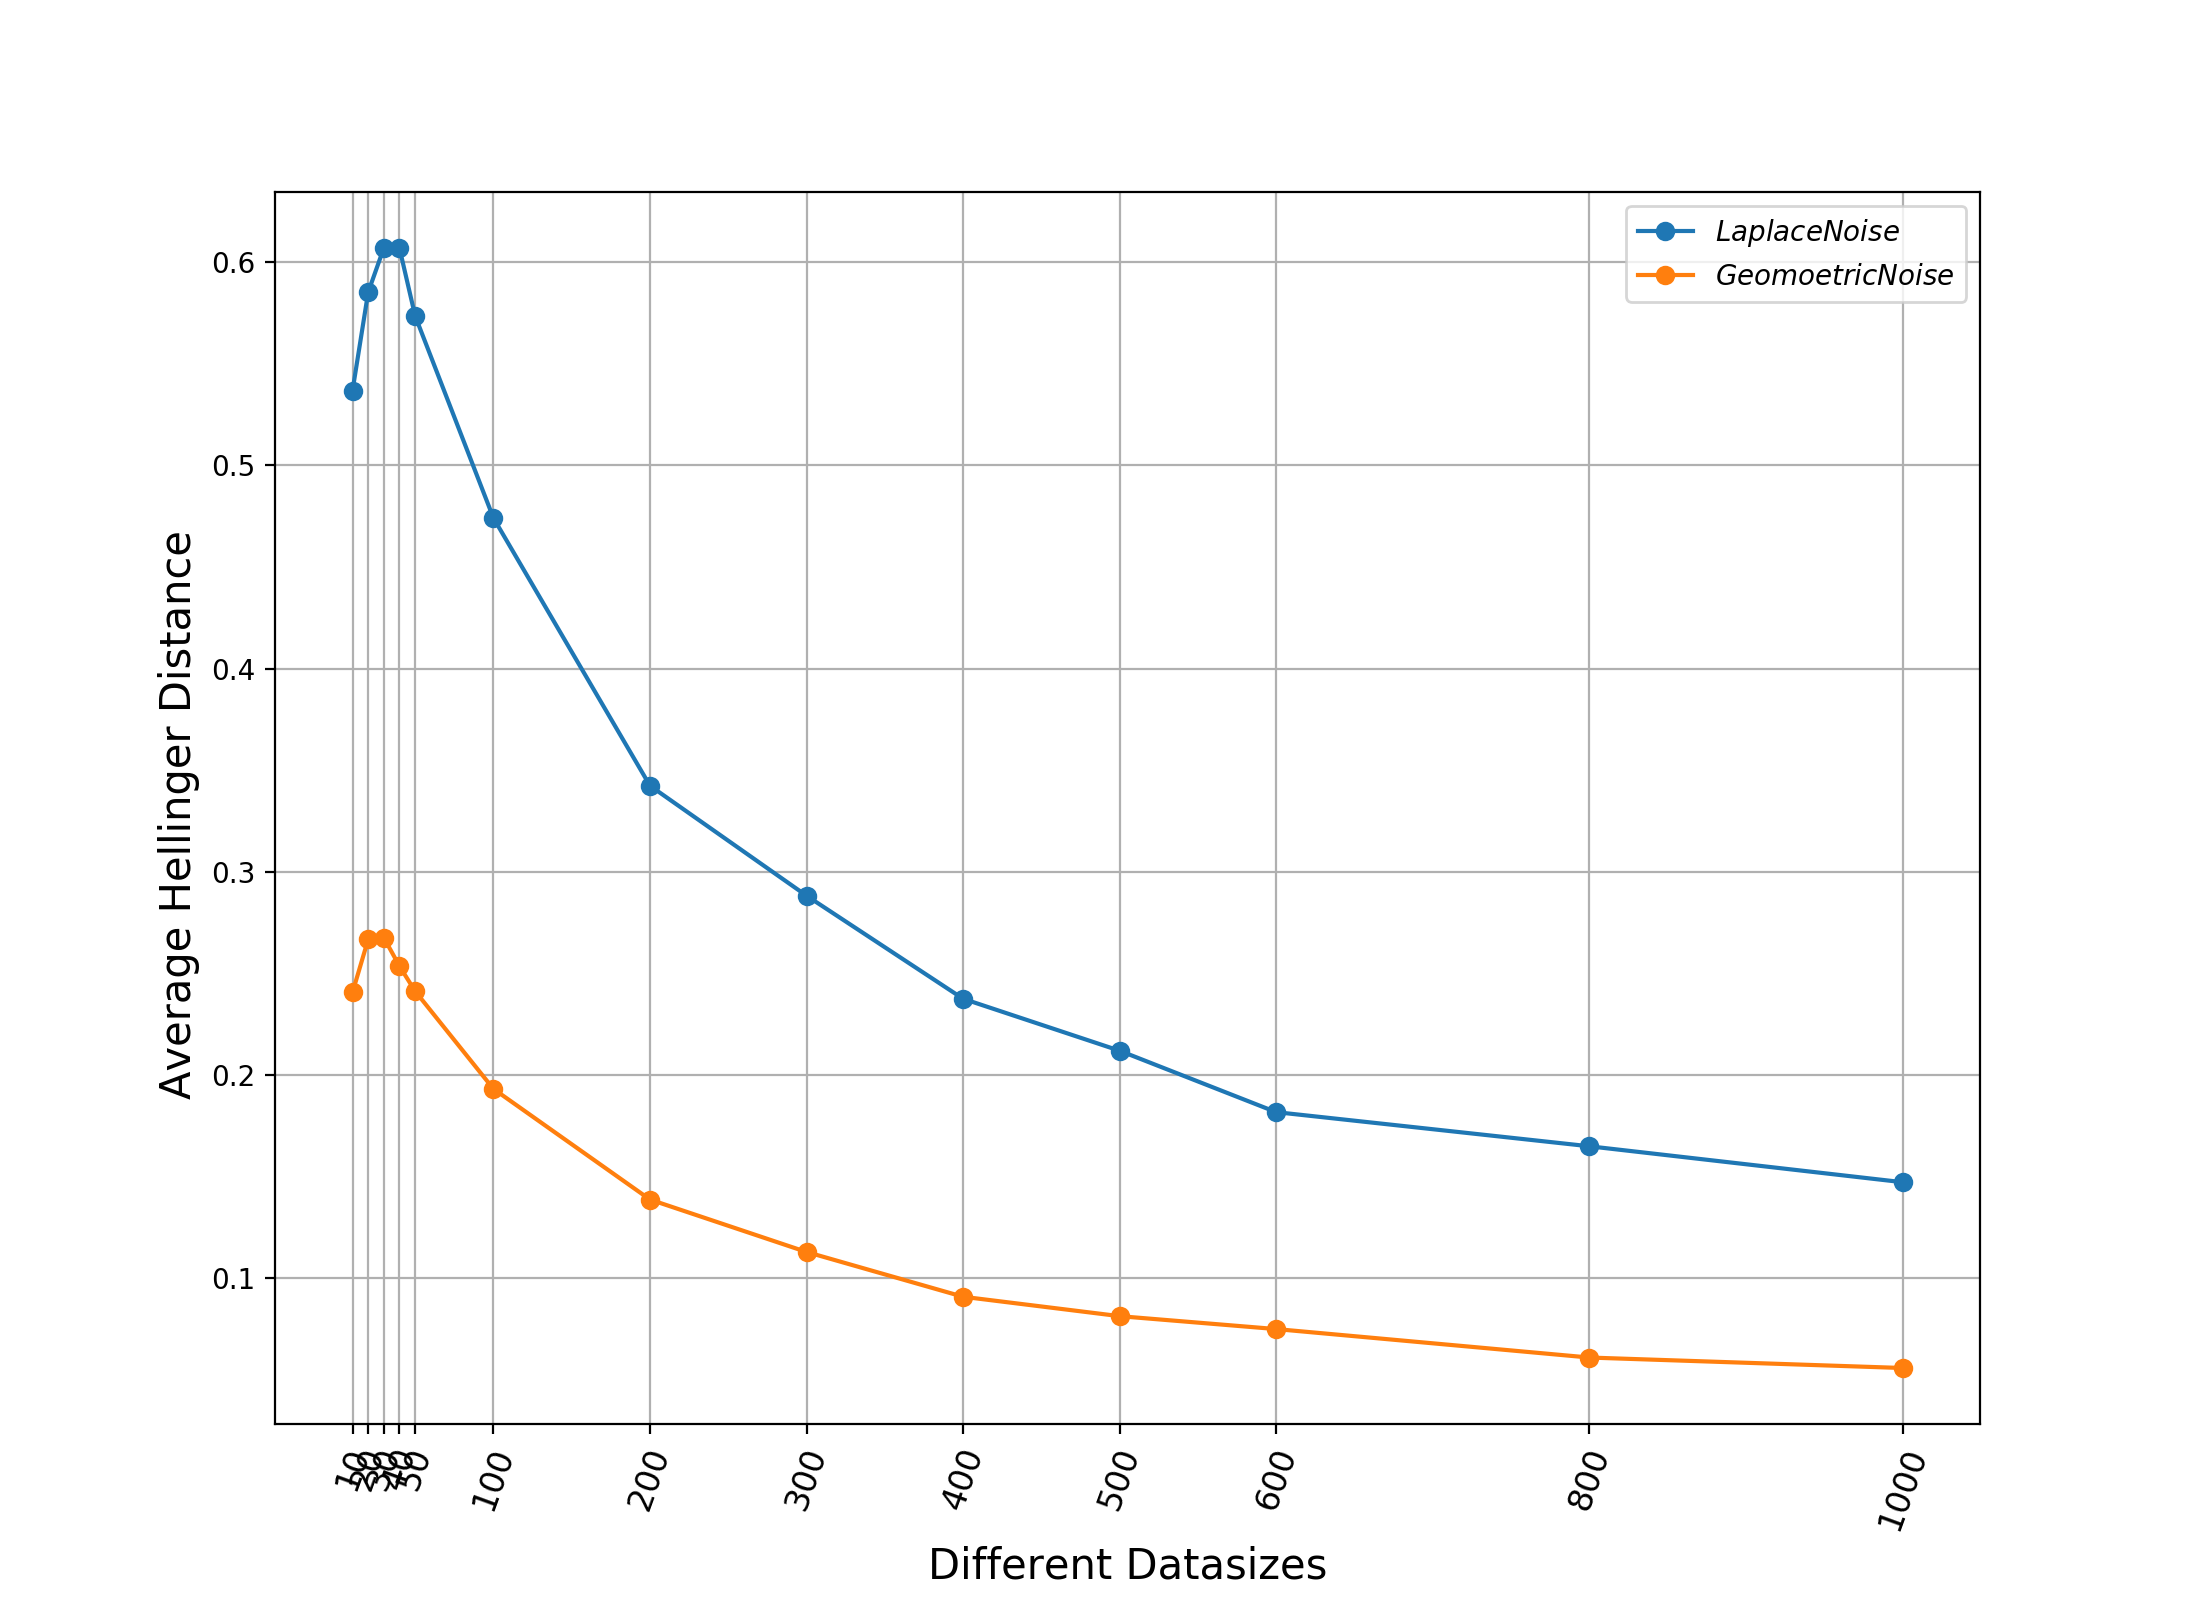
\includegraphics[height=1.2in]{datasize.png}
        \caption{Utility V.S. Different Data Sizes $n$, given $\epsilon = 0.1$}
    \end{subfigure}%
    ~ 
    \begin{subfigure}[t]{0.3\textwidth}
        \centering
        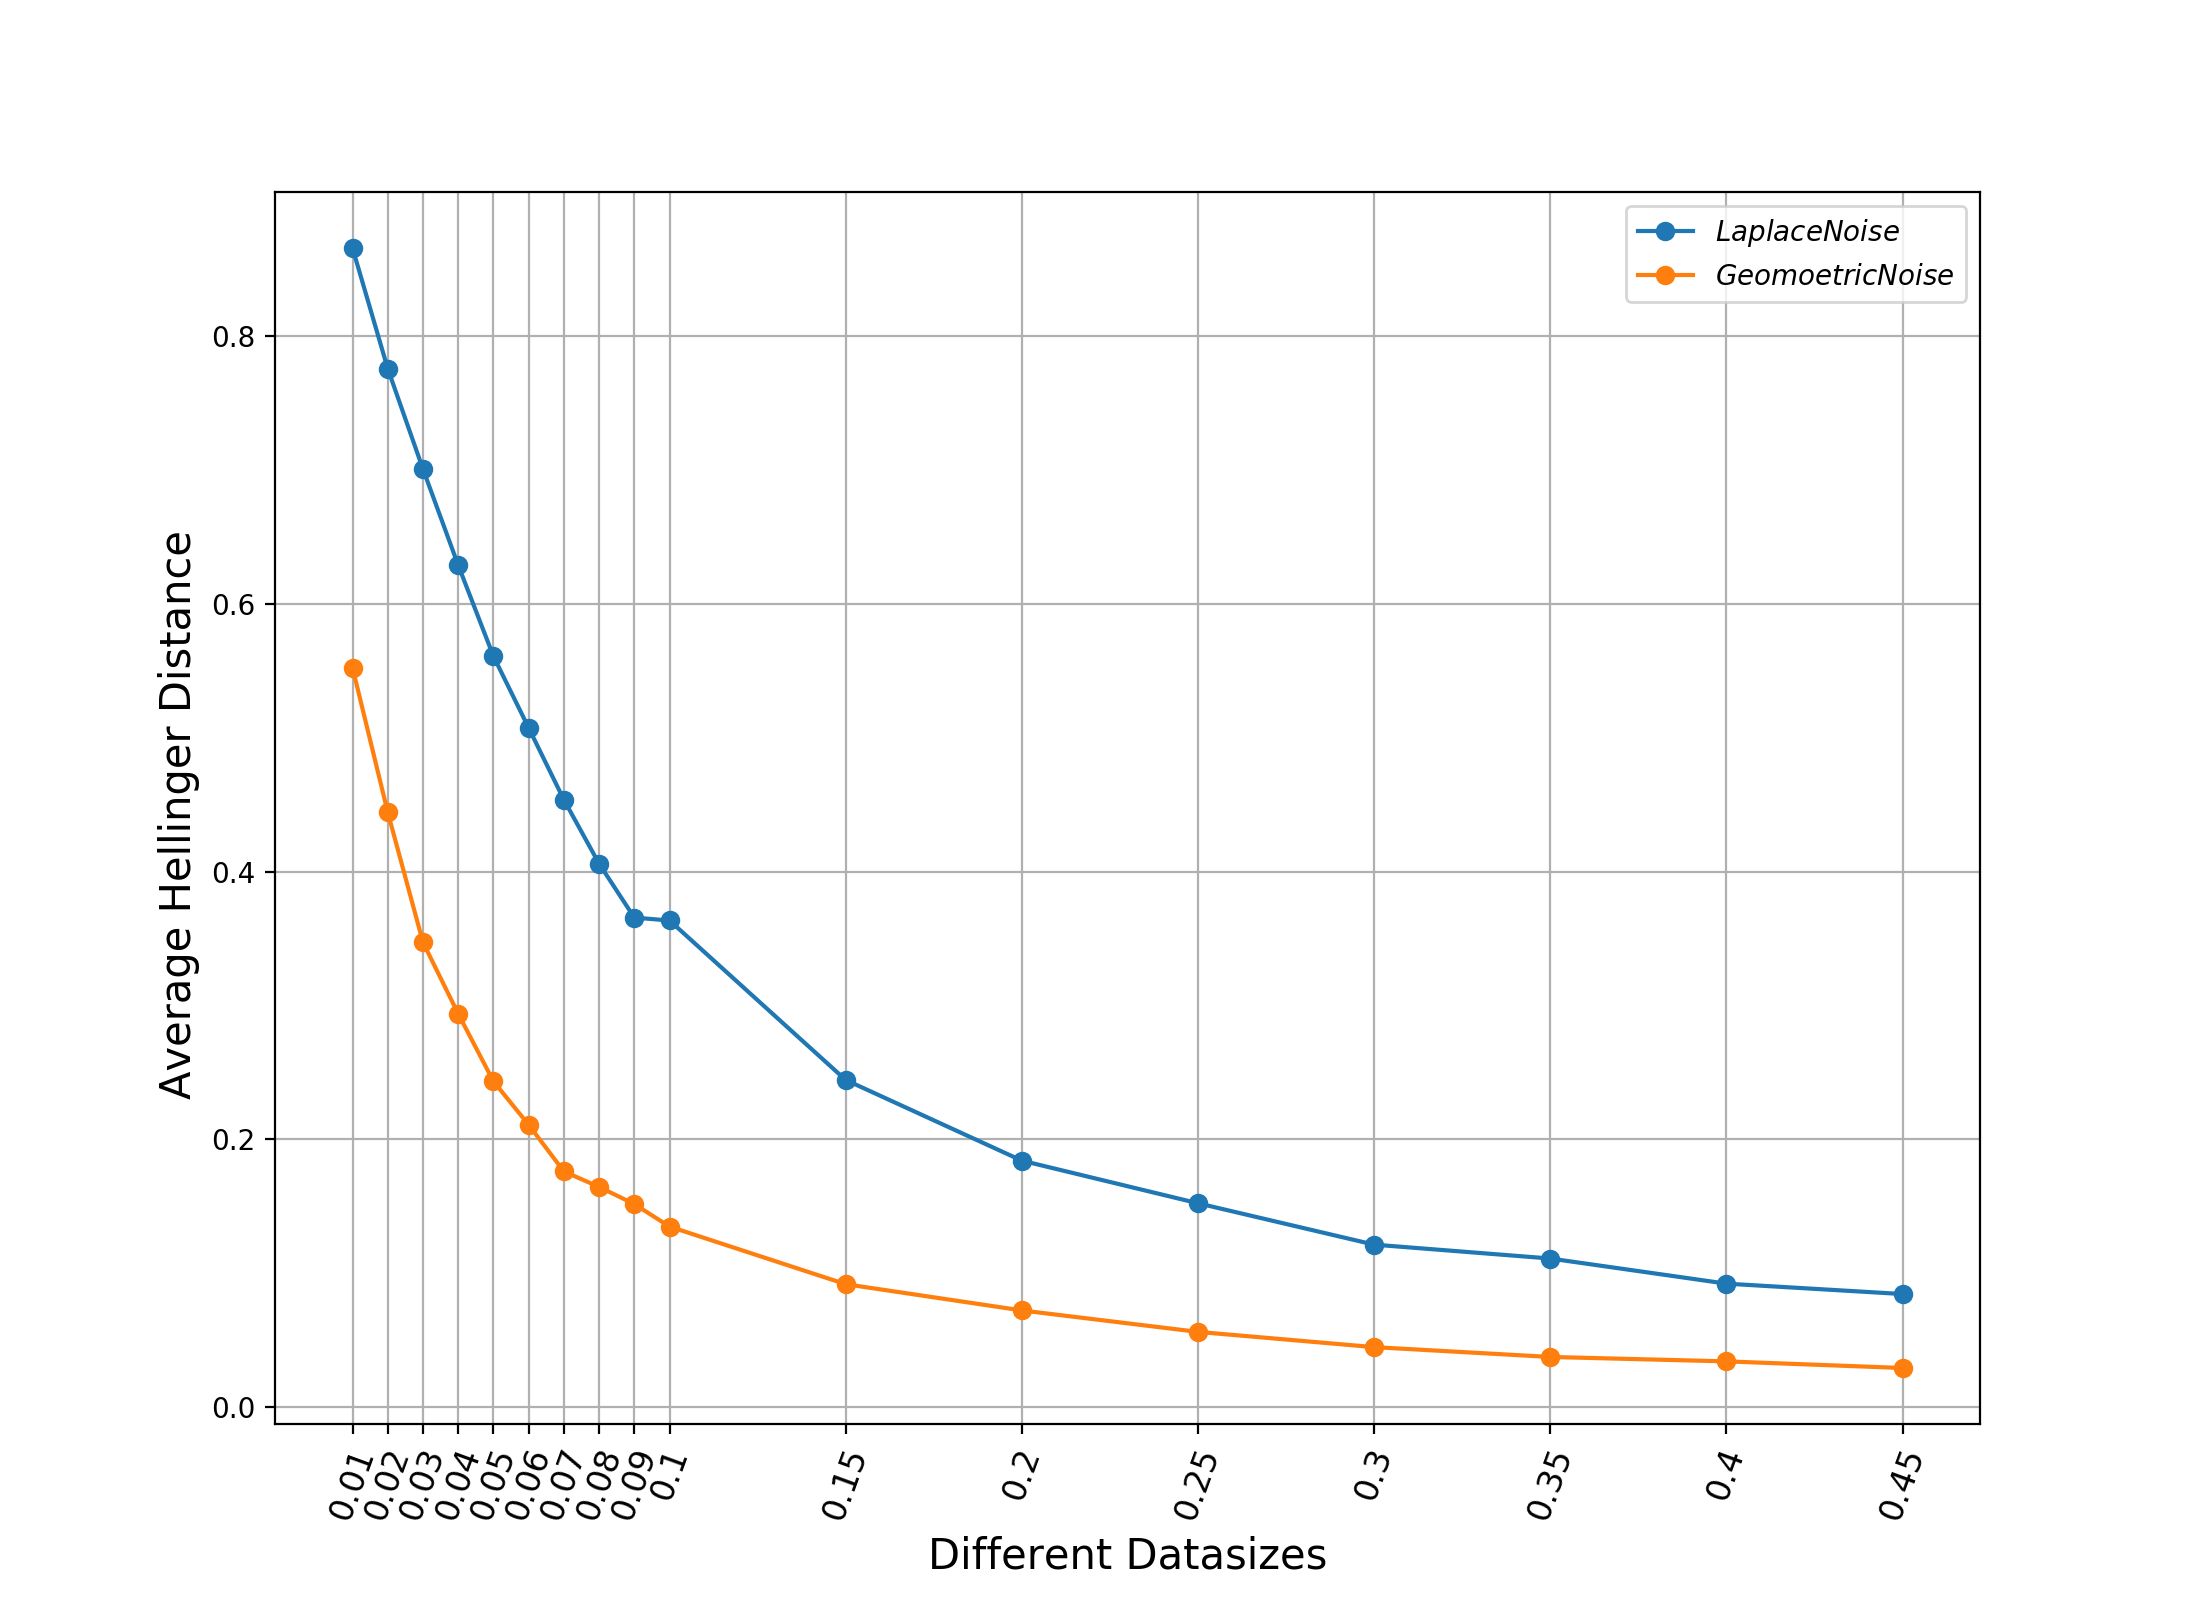
\includegraphics[height=1.2in]{eps_size200}
        \caption{Utility V.S. Different $\epsilon$ given data size $n = 200$}
    \end{subfigure}
    ~ 
    \begin{subfigure}[t]{0.3\textwidth}
        \centering
        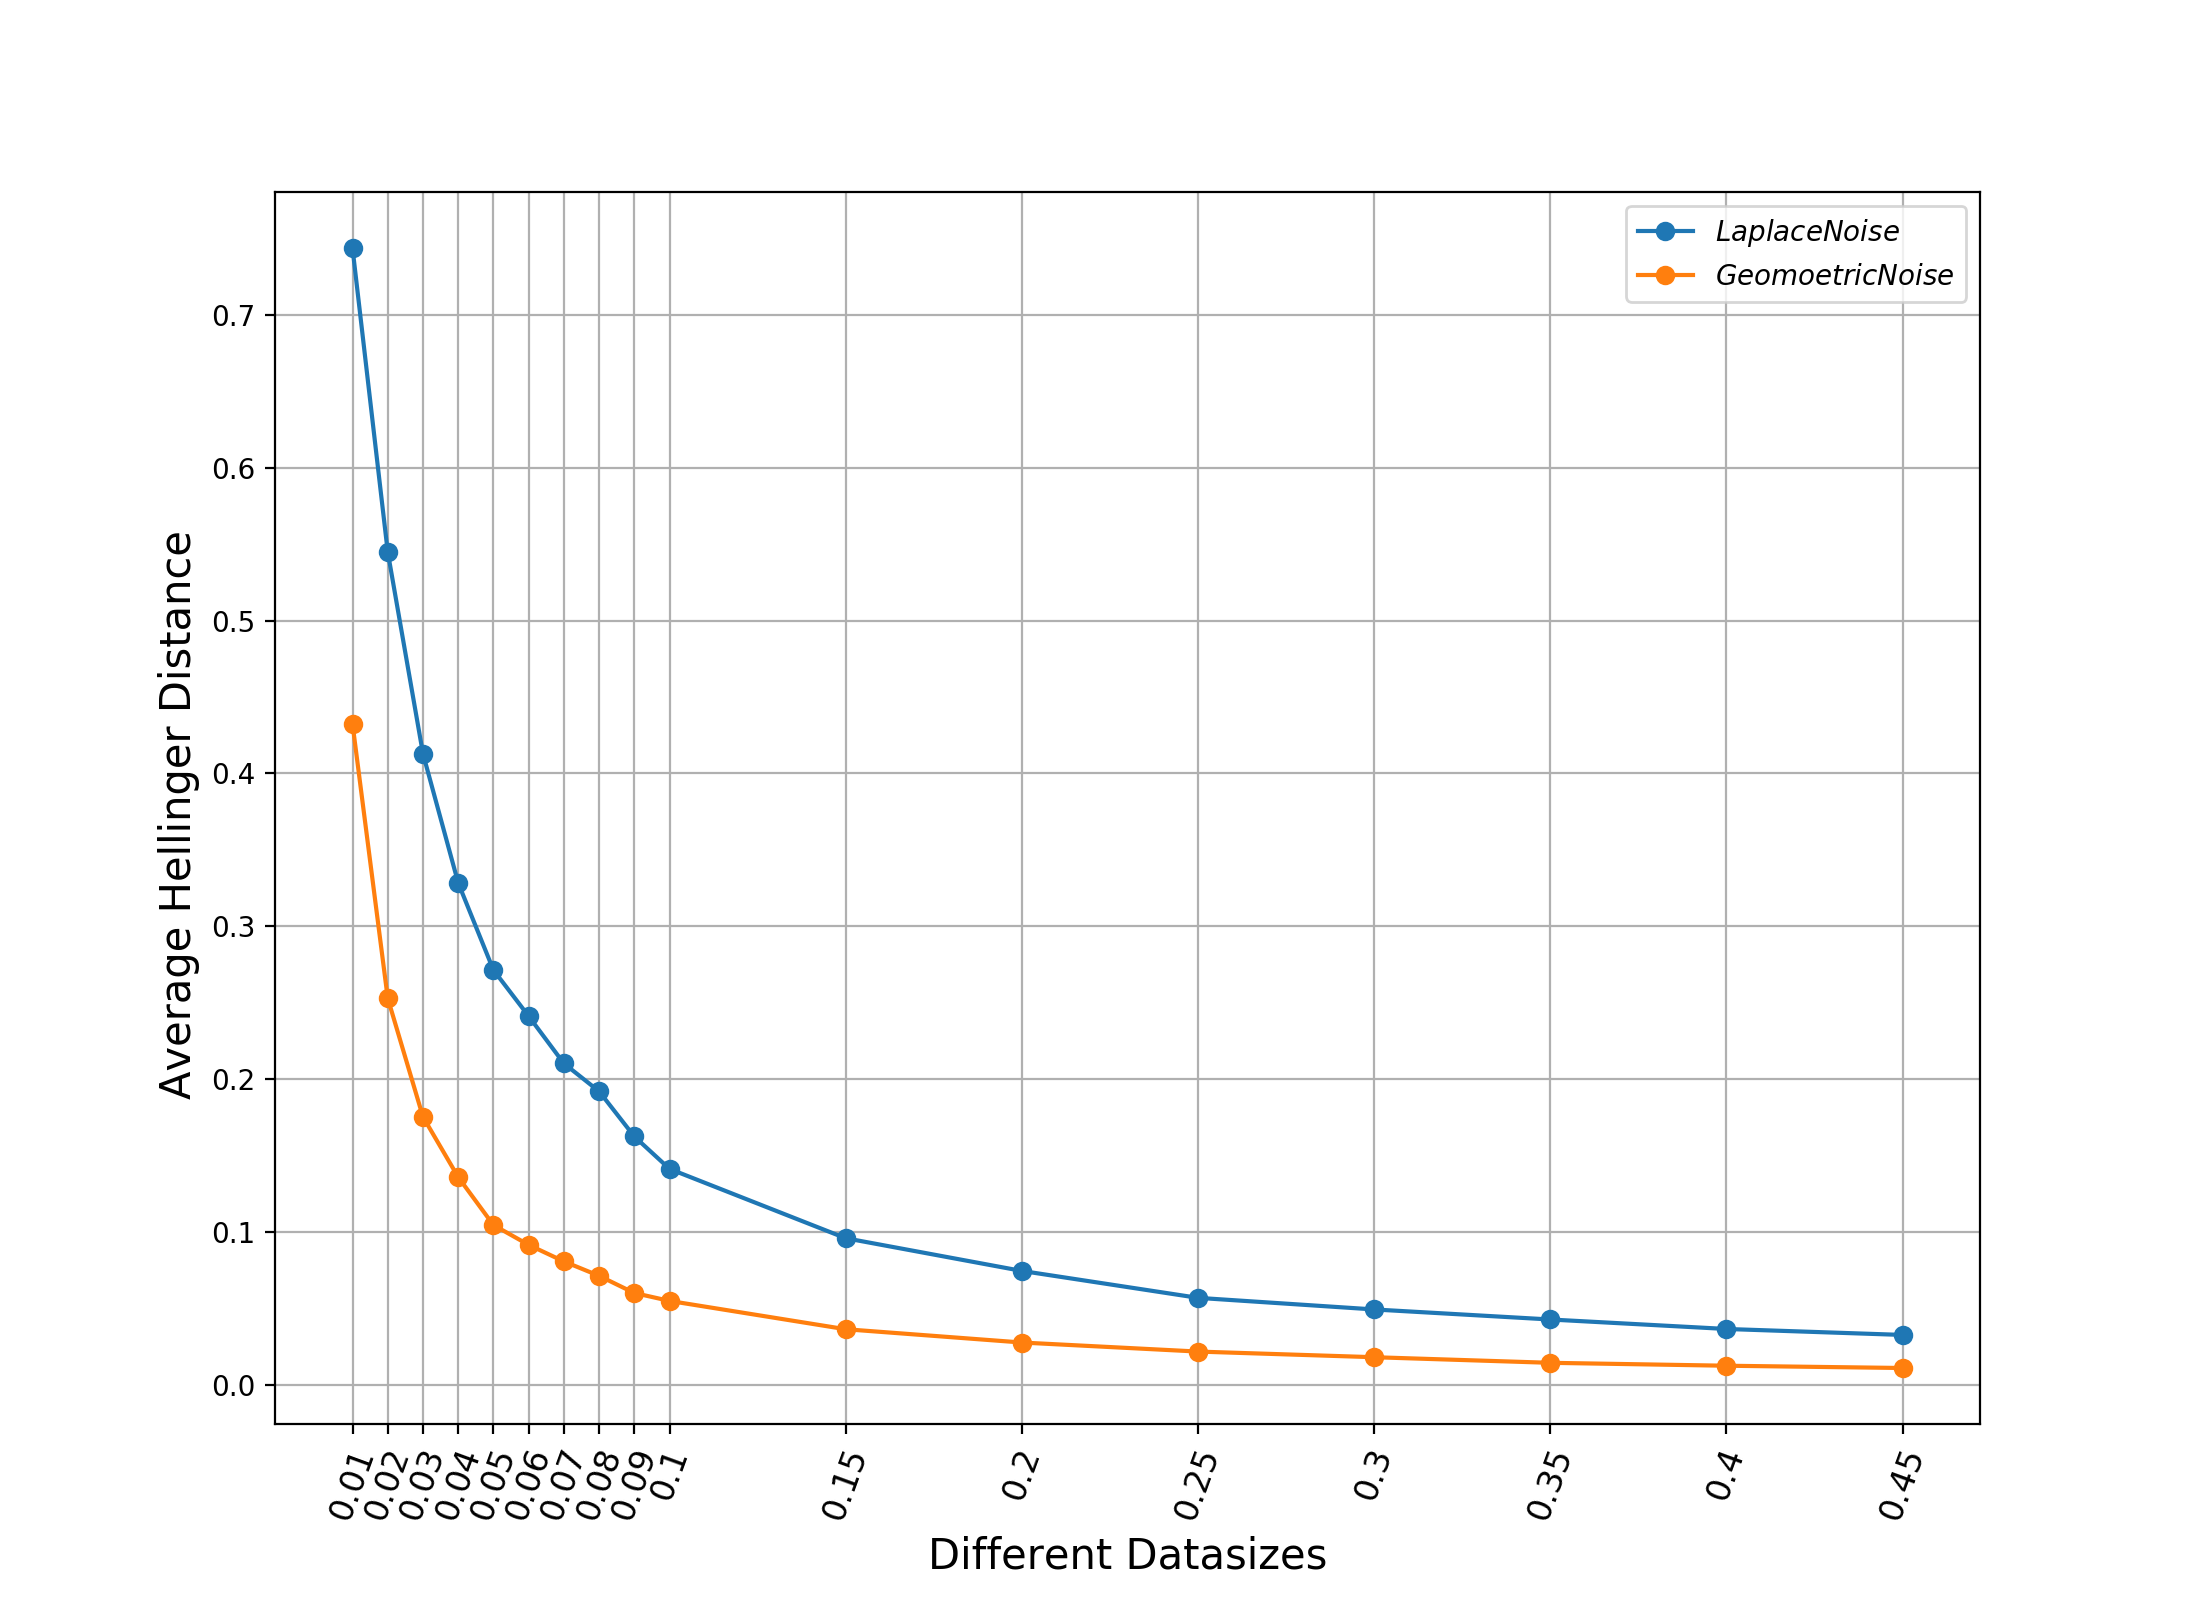
\includegraphics[height=1.2in]{eps_size1000}
        \caption{Utility V.S. Different $\epsilon$ given data size $n = 1000$}
    \end{subfigure}
    \caption{Utility of two different models}
    \label{fig_geovslap}
\end{figure*}
%

\section{Conclusion}
The summary of existing structures of DP-Bayesian inference works can help to develop some fundamental frameworks in this line. Then, the study of the connections between different utility optimality, and their common utility properties can help to develop new optimality for some other differentially private Bayesian work that haven't achieve optimality. This project will even build the framework for the differentially private Bayesian inference.

\section*{Appendix}
Code is available also in github \url{https://github.com/jiawenliu/CS591S1.git}.


\begin{lstlisting}[label=code-alg2, language=Python, caption=Python Code For Algorithm 2 Simple Histogram CDF]
import numpy as np
import matplotlib.pyplot as plt
import math

#############################################################################
#GENERATING DATA SIZE AND CONRRESPONDING PARAMETER
#############################################################################

def gen_dataset(n):
	data = []
	for _ in range(n):
		x = np.random.normal(0.7, 0.01)
		data.append(0.0 if x < 0.0 else 0.99 if x > 1.0 else x)

	return np.array(data)

def gen_datasizes(r, step):
	return [i*step for i in range(r[0]/step,r[1]/step + 1)]

#############################################################################
#SETTING UP THE GRANULARITY OF T
#############################################################################

def gen_t():
	return [0.1 * i for i in range(10)]

#############################################################################
#SIMPLE HISTOGRAM ALGORITHM
#############################################################################
def Simple_Histogram(x, a, eps):
	Y = [0]
	n = len(x)
	for j in range(1, int(1/a) + 1):
		I0, I1 = (j - 1) * a, j * a
		count = 0
		for xi in x:
			count += 1 if (xi < I1 and xi >= I0) else 0.0
		Y.append(count/n + np.random.laplace(0.0, 2/(eps * n)))
	return Y

#############################################################################
#SIMPLE HISTOGRAM CDF ALGORITHM
#############################################################################
def Simple_Histogram_CDF(x, a, eps):
	Y = Y = Simple_Histogram(x, a, eps)
	n = len(x)
	def eCDF(t):
		return sum([Y[j] for j in range(1, int(math.floor(t/a)))]) + (t/a - math.floor(t/a)) * Y[int(math.floor(t/a)) + 1]
	
	ecdf = np.array([eCDF(t) for t in gen_t()])

	return Y, ecdf

#############################################################################
# CDF FUNCTION
#############################################################################
def CDF(x):
	n = len(x)
	def CDFt(t):
		count = 0.0
		for xi in x:
			if xi < t: count += 1.0
		return count/n
	return np.array([CDFt(t) for t in gen_t()])


#############################################################################
# ERROR COMPUTING
def error(cdf, ecdf):
	return max(abs(cdf - ecdf))

#############################################################################
# TEST SIMPLE OR TREE CDF FUNCTION
def expermt(eps, n, a):
	e = 0.0
	for _ in range(20):
		x = gen_dataset(n)
		Y, ecdf = Simple_Histogram_CDF(x, a, eps)
		cdf = CDF(x)
		e += error(cdf, ecdf)
	print a, e
	return e/20.0

def expermt_va(eps, n, va):
	return [expermt(eps, n, a) for a in va]

def plot_accuracy(ys, ns):
	plt.figure()
	plt.plot(ns, ys, "ro-", label = "Error")
	plt.xlabel(r'$\alpha = \frac{1}{2^{x}}$')
	plt.ylabel("Error")
	plt.title(r"Simple Histogram CDF with n = $10^5$")
	plt.legend()
	plt.grid()
	plt.show()

if __name__ == "__main__":
	#############################################################################
	#SETTING UP THE PARAMETERS WHEN DOING GROUPS EXPERIMENTS
	#############################################################################
	eps = 0.5
	n = 100000
	va = [(1.0/2) ** i for i in range(1, 16)]
	plot_accuracy(expermt_va(eps, n, va), range(1, 16))

\end{lstlisting}

\begin{lstlisting}[label=code-alg3, language=Python, caption=Python Code For Algorithm 2 Tree Histogram CDF]
import numpy as np
import matplotlib.pyplot as plt
import math

#############################################################################
#GENERATING DATA SIZE AND CONRRESPONDING PARAMETER
#############################################################################

def gen_dataset(n):
	data = []
	for _ in range(n):
		x = np.random.normal(0.7, 0.01)
		data.append(0.0 if x < 0.0 else 0.99 if x > 1.0 else x)

	return np.array(data)

def gen_datasizes(r, step):
	return [i*step for i in range(r[0]/step,r[1]/step + 1)]

#############################################################################
#SETTING UP THE GRANULARITY OF T
#############################################################################

def gen_t():
	return [0.1 * i for i in range(10)]


#############################################################################
#SIMPLE HISTOGRAM ALGORITHM
#############################################################################
def Simple_Histogram(x, a, eps):
	Y = [0]
	n = len(x)
	for j in range(1, int(1/a) + 1):
		I0, I1 = (j - 1) * a, j * a
		count = 0
		for xi in x:
			count += 1 if (xi < I1 and xi >= I0) else 0.0
		Y.append(count/n + np.random.laplace(0.0, 2/(eps * n)))
	return Y



#############################################################################
#TREE HISTOGRAM CDF ALGORITHM
#############################################################################
def Tree_Histogram_CDF(x, eps, l):
	va = [(1.0/2) ** i for i in range(1, l)]
	vY = [ Simple_Histogram(x, a, eps) for a in va]
	def eCDF(t):
		d = np.argmin(np.array([(t/a - math.floor(t/a)) for a in va]))
		Y, a = vY[d], va[d]
		return sum([Y[j] for j in range(1, int(math.floor(t/a)))]) + (t/a - math.floor(t/a)) * Y[int(math.floor(t/a)) + 1]
	ecdf = np.array([eCDF(t) for t in gen_t()])

	return ecdf

#############################################################################
# CDF FUNCTION
#############################################################################
def CDF(x):
	n = len(x)
	def CDFt(t):
		count = 0.0
		for xi in x:
			if xi < t: count += 1.0
		return count/n
	return np.array([CDFt(t) for t in gen_t()])


#############################################################################
# ERROR COMPUTING
def error(cdf, ecdf):
	return max(abs(cdf - ecdf))

#############################################################################
# TEST SIMPLE OR TREE CDF FUNCTION
def expermt(eps, n, a):
	e = 0.0
	for _ in range(20):
		x = gen_dataset(n)
		Y, ecdf = Tree_Histogram_CDF(x, a, eps)
		cdf = CDF(x)
		e += error(cdf, ecdf)
	print a, e
	return e/20.0

def expermt_va(eps, n, va):
	return [expermt(eps, n, a) for a in va]

def plot_accuracy(ys, ns):
	plt.figure()
	plt.plot(ns, ys, "ro-", label = "Error")
	plt.xlabel(r'$\alpha = \frac{1}{2^{x}}$')
	plt.ylabel("Error")
	plt.title(r"Tree Histogram CDF with n = $10^3$")
	plt.legend()
	plt.grid()
	plt.show()

if __name__ == "__main__":
	##############################################################
	#SETTING UP THE PARAMETERS WHEN DOING GROUPS EXPERIMENTS
	#############################################################
	eps = 0.5
	n = 1000
	vl = range(1, 16)
	plot_accuracy(expermt_va(eps, n, va), range(1, 16))

\end{lstlisting}






\newpage
\bibliographystyle{plain}
\bibliography{main.bib}



\end{document}
